\newif\ifRAL
% Comment one of the following lines
\RALtrue 	% RAL PAPER
%\RALfalse 	% ICRA PAPER

\newif\ifTR
% Comment one of the following lines
%\TRtrue 	% Tech report in
\TRfalse 	% Tech report not in

\newif\ifPrePrint
%\PrePrinttrue
\PrePrintfalse

\ifRAL
  \documentclass[letterpaper, 10 pt, journal, twoside]{IEEEtran}
\else
  \documentclass[letterpaper, 10 pt, conference]{ieeeconf}
\fi

% This command is only
% needed if you want to
% use the \thanks command
\IEEEoverridecommandlockouts

\ifRAL
	% \overrideIEEEmargins
	% Comment this command for final RAL version.
	% Use this command for initial and revised RAL versions, and for final conference version
\else
% See the \addtolength command later in the file to balance the column lengths
% on the last page of the document
	\overrideIEEEmargins
	\def\baselinestretch{0.99}
\fi		


% save and then undefine the offending command
% we need \makeatletter because \@undefined uses the special @ character.
\makeatletter
\let\IEEEproof\proof
\let\IEEEendproof\endproof
\let\proof\@undefined
\let\endproof\@undefined
\makeatother




% See the \addtolength command later in the file to balance the column lengths
% on the last page of the document
\usepackage{scrextend}
\usepackage[hidelinks]{hyperref}
\usepackage{graphicx}   % for pdf, bitmapped graphics files
\usepackage{epsfig}    % for postscript graphics files
\usepackage{amsmath}    % assumes amsmath package installed
\usepackage{amssymb}    % assumes amsmath package installed
\usepackage{mathtools}  % assumes amsmath package installed
\usepackage{float}
\usepackage{booktabs,tabularx}
\usepackage[caption=false]{subfig}
% for compact citation of multiple authors
\usepackage{cite}
\usepackage{accents}
% for blank spaces
\usepackage{blindtext}
\usepackage{xcolor}
 % used for the two-column index
\usepackage{multicol}       
\usepackage{booktabs,tabularx}
\usepackage{multirow}
\usepackage{accents}
\newcommand{\ubar}[1]{\underaccent{\bar}{#1}}

\let\proof\relax
\let\endproof\relax
\usepackage{amsthm}
\newtheorem{definition}{Definition}
\newtheorem{problem}{Problem}
\newtheorem{remark}{Remark}
\newtheorem{note}{Note}
\newtheorem{assumption}{Assumption}

\usepackage{multicol}
\usepackage{xcolor}
%% general definitions
\newcommand\AF[1]{{\textcolor{red}{AF:#1}}}


\let\labelindent\relax
\let\labelindent\relax
\usepackage{enumitem}
\newcommand{\subscript}[2]{$#1 _ #2$}

\DeclareMathOperator{\atantwo}{atan2}
\DeclareMathOperator{\asin}{asin}



% \\\\\\\ Title \\\\\\
\ifRAL % RAL
	\title{ Towards Safe Human-Quadrotor Interaction: Mixed-Initiative Control Algorithm Using Real-Time NMPC}

\else % ICRA
	\title{\bf Towards Safe Human-Quadrotor Interaction: Mixed-Initiative Control Based on Real-Time NMPC}
\fi



\author{B\'arbara Barros Carlos$^{1}$, Antonio Franchi$^{2}$ and Giuseppe Oriolo$^{1}$% <-this % stops a space
%\thanks{*This work was not supported by any organization}% <-this % stops a space
\thanks{$^{1}$B. B. Carlos and G. Oriolo are with the Department of Computer, Control \& Management Engineering (DIAG), Sapienza Universit\`a di Roma, Italy.
        {\tt\footnotesize \{barros, oriolo\}@diag.uniroma1.it}}%
\thanks{$^{2}$A. Franchi is with the University of Twente, 
Faculty of Electrical Engineering, Mathematics \& Computer Science,  Robotics and Mechatronics Laboratory, The Netherlands and also with LAAS-CNRS, CNRS, Universit\'e de Toulouse, France
        {\tt\footnotesize a.franchi@utwente.nl}}%
\thanks{This work is partially funded by the European Commission project H2020 AERIAL-CORE (EC 871479).}%
}

\begin{document}

\maketitle
\thispagestyle{empty}
\pagestyle{empty}

%===============================================================================
\begin{abstract}
This paper presents a novel algorithm for blending human inputs and motion generator commands, guaranteeing safety in mixed-initiative interactions between humans and quadrotors. The algorithm is based on nonlinear model predictive control (NMPC) and involves using the state solution to assess whether safety- and/or task-related rules are met to mix control authority. The mixing is attained through the convex combination of human and actual robot costs, driven by a continuous function that measures the violation of the rules. To achieve real-time feasibility, we rely on an efficient real-time iteration (RTI) variant of a sequential quadratic programming (SQP) scheme to cast the mixed-initiative controller. We demonstrate the effectiveness of our algorithm through numerical simulations, where a second autonomous algorithm is used to emulate the behavior of pilots with different competence levels. Simulations show that our scheme provides suitable assistance to pilots, especially novices, in a workspace with obstacles while underpinning computational efficiency. 
\end{abstract}
%===============================================================================
\section{INTRODUCTION}
Quadrotors have been widely used across various applications, resulting in a significant market expected to grow exponentially. Due to this increasing demand, one can envisage that, in the future, learning to fly a quadrotor will become a taken-for-granted skill, just as learning to drive a car nowadays. A first step could be a mixed-initiative control approach that guarantees the aerial system's ``working conditions" while the novice operator learns to fly it. In other words, as long as some safety- and/or task-related rules are met, the operator commands are obeyed. Once novices start working in the context of complex tasks, it is essential to provide them with the assistance that gradually decreases as their competence increases -- here, competence refers to the knowledge and ability that allow the use of the robot to accomplish a task. Conversely, one could think of an experienced operator who already has the competence level that enables him/her to fly a quadrotor. But as his/her cognitive load is primarily focused on the short-term aspect of the task, he/she cannot consider other underlying factors in the long run (e.g., safety). It is then essential to have a control approach that supervises the task in the long term to prevent the operator from being overwhelmed by (too) high engagement.  

To fill these gaps, in this paper, we propose an efficient mixed-initiative controller based on nonlinear model predictive control (NMPC) to enforce safety in human-quadrotor interactions. The technical difficulties associated with the proposed controller are twofold: first, satisfy both the existing constraints and the human intentions; second, solve the underlying optimization problems that include a high-dimensional quadrotor system under the available computation time. We demonstrate how to handle these difficulties using concepts of zone MPC and online weight adaptation within the real-time iteration (RTI) scheme, an efficient Newton-type algorithm for real-time NMPC applications. To further speed-up solution times, we exploit high-performance numerical optimization algorithms, structure-exploiting convex solver, and linear algebra library in our implementation. The mixed-initiative controller is validated in simulation, where an autonomous algorithm emulates the behavior of pilots with different competence levels. To the best of our knowledge, this is the first mixed-initiative controller that overcomes all aforenamed dilemmas. For this reason, this work makes a significant contribution to human-robot interaction literature.

\subsection{Related works}
One way robots and humans can interact is to put the human in the loop with some blending scheme \cite{amirshirzad2019}. In a nutshell, the human and the automatic controller have control over the robot, and both systems must adapt to ensure task completion. For example, in bimanual robot manipulation, the robot can arbitrate between the user's command inputs and its underlying motion policies and understanding of bimanual tasks \cite{rakita2019, xi2019}. In exoskeleton systems, the interplay between robot and human may be characterized as an interaction between teacher and student in a learning process. The teacher (robot) tries to minimize the student (human) error, applying a minimal effort \cite{bao2020, santos2019}. In the context of autonomous cars, the driver interacts with the automatic controller that aims at reducing the driver's workload and, at the same time, taking prompt actions in case of human failure \cite{huang2019, lu2019}. For human-swarm systems, the interaction paradigm is less obvious. As the size of the swarm increases, control should become more focused on the swarm as a whole rather than on the individuals, given the human's limited capacity to multitask. In this case, the interaction is more concerned with the human-swarm ability to accomplish a particular task than with the spatial positioning of the swarm \cite{ashcraft2019, nam2019}. 

Other interactive approaches rely on methods designed from the human perspective, where, in general, the presence of haptic cues increases situational awareness. These methods lean heavily in favor of perceiving the human as the source of action and the robot as the passive collaborator. For instance, virtual fixtures have been used to inform the operator of the highest comfort position, distance from the target position, or proximity to unsafe kinematic configurations \cite{rahal2020, abi2020}. Obstacle avoidance is one of the most critical requirements to be met in many robotics scenarios. In this matter, haptic feedback can help inform the operator of instantaneous collisions \cite{parsa2020, masone2018}. The work in \cite{franchi2017} compares several human-collaborative schemes, highlighting their main aspects where haptic feedback is one of those.

\subsection{Contributions and paper structure}
The main contributions of this work are twofold:
\begin{itemize}
	\item Novel mixed-initiative control algorithm for human-quadrotor systems based on real-time NMPC with safety guarantees.
	\item A numerical simulation that shows the computational efficiency and effectiveness of the proposed algorithm.
\end{itemize}

This paper is structured as follows. Section \ref{sec:problem_statement} states the problem we want to solve. Section \ref{sec:algo_details} provides the details of the proposed algorithm. The numerical simulations are described, and their results are discussed in Section \ref{sec:numerical_results}. Finally, the conclusion is made in Section \ref{sec:conclusion}.

\subsection{Notation}
Operations such as $x \leq y$ is understood to be element-wise, whereas $\max(x)$ is vector-wise. Vectors are column vectors and we use the notation $(x; y; z)$ to denote concatenation. It is denoted by $\mathbf{I_n}$ the set of $n \times n$ identity matrices. An all-ones vector of dimension $n$ is denoted by $\mathbf{1_n}$, whereas $\mathbf{0_n}$ denotes a $n$-vector of zeros. When dealing with norms of vectors $x \in \mathbb{R}^n$, we denote by $\|x\|$ the Euclidean norm. The set of positive real-valued vectors of dimension $n$ is denoted by $\mathbb{R}^n_{>0}$.
%===============================================================================
\section{PROBLEM STATEMENT}\label{sec:problem_statement}
The fundamental problem in mixed-initiative control is how to blend human inputs and automatic controller commands to realize the former as much as possible while always enforcing safety. In this context, the formulation of our problem hinges upon the following components:
\begin{itemize}
	\item A \emph{robot} represented by a particular nonlinear, time-varying system
\begin{equation}
	\dot{\xi} = f(\xi,u),\label{eq:robot_dynamics}
\end{equation}
subject to a set of constraints, where states, control inputs and dynamics are denoted by $\xi \in \mathbb{R}^{n_\xi}$, $u \in \mathbb{R}^{n_u}$ and $f \vcentcolon \mathbb{R}^{n_\xi} \times \mathbb{R}^{n_u} \rightarrow \mathbb{R}^{n_\xi}$, respectively. 
	\item Task variables denoted by $\eta = z(\xi)$ and described in $\mathbb{R}^{n_\eta}$. Typical examples are:
	\begin{itemize}
	\item a subset of the state variables (which may even coincide with the state itself), e.g., cartesian points.
	\item some nonlinear vector, e.g., kinematic map for some point of the robot.
	\end{itemize}
	\item A motion generator that provides the collision-free \emph{reference trajectory} $\eta^r \in \mathbb{R}^{n_\eta}$ for the task variables. It could be either a global planner or an autonomous controller.                                                                                                                                                                                                                                                                                                                                                                                                                                                                                                                                                                                                                                                                                                                                                                                                                                                                                                                                                                                                                                                                                                                                                                                                                                                                                                                                                                                                                                                                                                                                                                                                                                                                                                                                                                                                                                                                                                                                                                                                                                                                                                                                                                                                                                                                                                                                                                                                                                                                                                                                                                                                                                                         
	\item The human who specifies desired values to the control interface variables denoted by $\nu^r \in \mathbb{R}^{n_\nu}$. These values are henceforth called \emph{human inputs}. As the notation suggests, they are reference signals representing human intentions.
	\item A set of \emph{working conditions} defining the minimum requirements that the robot must meet to operate healthily. They can contain both safety rules (e.g., maximum kinetic energy, maximum dissipation, etc.) and/or task-related rules (e.g., the accuracy of end-effector positioning and orientation, etc.).
	\begin{assumption}
		Working conditions are defined such that the resulting set is convex.
	\end{assumption}
\end{itemize}
For this setting, we want to devise a \emph{mixed-initiative controller} that will attempt to execute human inputs as much as possible without compromising the working conditions and the set of constraints inherent to the robot's physical limitations. As we will see, in addition to the mixed-initiative controller itself, the control algorithm also includes a blending mechanism that predicts the violation of working conditions and lends most of the control authority to the most capable agent at any time.

Let us now delve into the case of safe human-quadrotor interaction. The human operates the quadrotor providing it with four inputs: the desired roll, pitch, $z$ angular rate, and total thrust. They are sent to the robot through a control interface, which is usually a joystick. Here, the working conditions concern safety that comes in the form of collision-free motions. Thus, for the human pilot to safely fly a quadrotor, he/she needs to perceive the surrounding cues and decide how to control the quadrotor by modifying the inputs above to avoid potential collisions. This job is always demanding for a novice, and in most cases, the quadrotor ends up crashing in the workspace \cite{xu2018}. That is why a mixed-initiative controller capable of guaranteeing safety during the learning process is of particular importance. Another key aspect of this process is repetition. Through repetition, the pilot can gradually reach a motor pattern that enables him/her to execute the task and increase his/her competence successfully. To that end, we assume that the human-quadrotor system must track a position reference repeatedly. This scenario will help us to illustrate the performance of our algorithm.   
  
%  A common physical limitation in quadrotor systems is that propellers can only generate bounded thrust. More sophisticated schemes include control at the rotor torque level yielding a high-dimensional state space that can be challenging to treat.
%===============================================================================
\section{MIXED-INITIATIVE CONTROL}\label{sec:algo_details}
The mixed-initiative controller perceives the human operator and the motion generator as two different agents having the same control rights. The blending mechanism can assess the working conditions' violation and mixes the commands so as the most capable agent has the most control authority at any given moment. An example is when the working conditions include safety rules in the form of collision-free motion, as in this paper. Suppose human inputs compromise the quadrotor's safety. In that case, a violation will be predicted, and the blending will be carried out so that the control authority is mainly given to the motion generator.

Overall, this controller can be seen as an assistive scheme for novice and experienced pilots. Whereas for the former, it allows the pilot to learn to fly a quadrotor without crashing it, for the latter, it introduces some level of disengagement that enables the pilot to fly a quadrotor manually without focusing on avoiding obstacles. 

\begin{figure}[t]
	\centering
	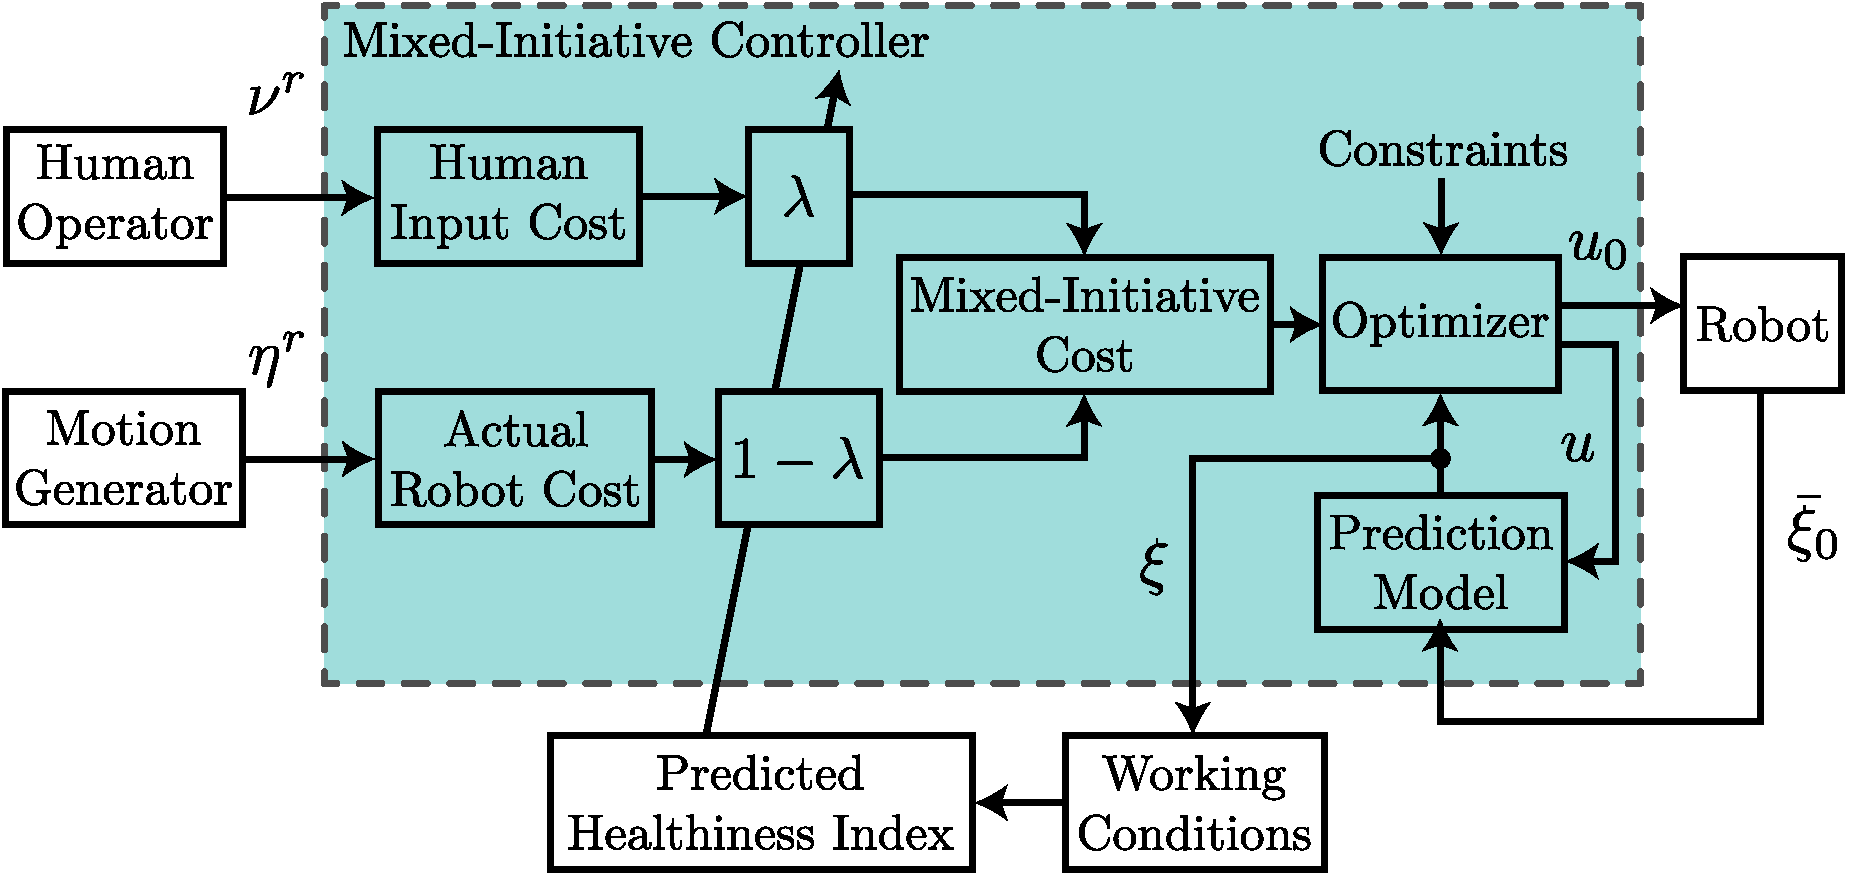
\includegraphics[width=0.49\textwidth]{figures/block_diagram}
	\vspace{-0.6cm}
	\caption{Block diagram summarizing the proposed mixed-initiative control algorithm present in Section \ref{sec:algo_details}.}\label{fig:block_diagram}%
\end{figure}

\subsection{Algorithm overview}
Mixed control is accomplished through a \emph{mixed-initiative NMPC controller} whose cost function -- the \emph{mixed-initiative cost}  -- is a convex combination between the \emph{actual robot cost} and the \emph{human input cost}. The latter is a cost term that penalizes the deviation from the human inputs. The  proposed blending mechanism is a continuous function between 0 and 1, named \emph{predicted healthiness index}, that drives the convex combination. It is computed in this way: when the index tends to 0, the working conditions' violation is too close and, hence, the mixed-initiative cost tends to the actual robot cost. When the index tends to 1, the violation is far enough and, therefore, the mixed-initiative cost tends to the human input cost.

Based on the state solution of the NMPC controller, at each time instant, the predicted healthiness index computes how far the robot is from violating the working conditions within a \emph{virtual horizon} whose length is defined by the designer. It then selects a value between 0 and 1 and blends the commands. The idea is that the closer the index to 0, the more troublesome it will be to keep the system within the working conditions in the next virtual horizon, even if full control is given to the motion generator (and human inputs are heavily ignored from that moment on). Vice-versa, the closer the index to 1, the easier the motion generator's job will be in case it takes full control of the system.  Fig.~\ref{fig:block_diagram} shows a block diagram of the proposed algorithm.
\subsection{Mixed-initiative controller}\label{subsec:nlps}
We regard the nonlinear program (\textbf{NLP$_1$}) corresponding to the constrained optimization problem of the low-level NMPC as follows:
\begin{equation*}\label{eq:nlp1}
{\!\!\!\!\!}{\!\!}\begin{aligned}
&\underset{\begin{subarray}{c}
\xi_0, \dots, \xi_N, \\
u_0, \dots, u_{N-1}
\end{subarray}}{\min}	    &&\frac{1}{2}\sum_{i=0}^{N-1} \|\eta(\xi_i, u_i)-\Bar{\eta}\|^2_{W} + \frac{1}{2}\|\eta_N(\xi_N)- \Bar{\eta}_N\|^2_{W_N}\\ 
&\,\,\,\quad \text{s.t.}    &&\xi_0 = \Bar{\xi}_0, \\
& 						    &&\xi_{i+1} - F_1(\xi_i,u_i) = 0, \,\,\,\,\,\, i = 0,\dots, N-1,\\
& 						    &&\Omega_i\in \mathbb{E}, \,\,\,\,\,\,\,\,\,\,\,\,\,\,\,\,\,\,\,\,\,\,\,\,\,\,\,\,\,\,\,\,\,\,\,\,\,\,\,\,\, i = 0,\dots, N-1,\\
& 						    &&u_i\in \mathbb{U}, \,\,\,\,\,\,\,\,\,\,\,\,\,\,\,\,\,\,\,\,\,\,\,\,\,\,\,\,\,\,\,\,\,\,\,\,\,\,\,\,\,\, i = 0,\dots, N-1,
\end{aligned}{\!\!\!}
\end{equation*}
\textcolor{red}{AF: shouldn't the desired state $\Bar{\eta}$ depend on $i$ since it is time varying? Also please make it clear from the beginning, in the problem setting, that this is a trajectory that is passed to the system by an external planner in order to execute the task.}
where $\xi \in \mathbb{R}^{n_{\xi}}$ and $u \in \mathbb{R}^{n_u}$ denote the state and input trajectories of the discrete-time robot system whose dynamics are described by $F_1 \vcentcolon \mathbb{R}^{n_{\xi}} \times \mathbb{R}^{n_u} \rightarrow \mathbb{R}^{n_{\xi}}$. The residuals in the stage and terminal least-squares terms are denoted by $\eta \vcentcolon \mathbb{R}^{n_{\xi}} \times \mathbb{R}^{n_u} \rightarrow \mathbb{R}$ and $\eta_N \vcentcolon \mathbb{R}^{n_{\xi}} \rightarrow \mathbb{R}$, and will be penalized by the symmetric positive-definite matrices $W$ and $W_N$, respectively. The output variables $\Bar{\eta} \vcentcolon \mathbb{R}^{n_{\xi}} \times \mathbb{R}^{n_u} \rightarrow \mathbb{R}$ and $\Bar{\eta}_N \vcentcolon \mathbb{R}^{n_{\xi}} \rightarrow \mathbb{R}$ represent the time-varying references passed to the automatic controller. We denote the admissible sets of $u$ and $\Omega$ as $\mathbb{U} \vcentcolon = [\ubar{u}, \Bar{u}]$ and $\mathbb{E} \vcentcolon = [\ubar{\Omega}, \Bar{\Omega}]$, where the bounds $\ubar{u}$, $\Bar{u}$, $\ubar{\Omega}$, and $\Bar{\Omega}$ are given. Finally, $N$ and $\Bar{\xi}_0$ denote the horizon length and the current state of the system, respectively. 

\textcolor{red}{AF: Another general comment I have is that I am not sure that making the difference between Euler angles is mathematically correct, anyway let's go back to this later.}

Similarly, the nonlinear program (\textbf{NLP$_2$}) that corresponds to the constrained optimization problem of the zone NMPC is:
\begin{equation*}\label{eq:nlp2}
{\!\!\!\!\!}{\!\!}\begin{aligned}
&\underset{\begin{subarray}{c}
\sigma_0, \dots, \sigma_N, \\
u_0, \dots, u_{N-1}
\end{subarray}}{\min}	    &&\frac{1}{2}\sum_{i=0}^{N-1} \|\eta(\sigma_i,u_i)-\Tilde{\eta}\|^2_{W(\epsilon_i^ \star)} + \frac{1}{2}\|\eta_N(\sigma_N)-\Tilde{\eta}_N\|^2_{W_N(\epsilon_i^\star)}\\ 
&\,\,\,\quad \text{s.t.}    &&\sigma_0 = \Bar{\sigma}_0, \\
& 						    &&\sigma_{i+1} - F_2(\sigma_i,u_i) = 0, \,\,\,\,\,\, i = 0,\dots, N-1,\\
& 						    &&\Omega_i\in \mathbb{E}, \,\,\,\,\,\,\,\,\,\,\,\,\,\,\,\,\,\,\,\,\,\,\,\,\,\,\,\,\,\,\,\,\,\,\,\,\,\,\,\,\,\,\, i = 0,\dots, N-1,\\
& 						    &&u_i\in \mathbb{U}, \,\,\,\,\,\,\,\,\,\,\,\,\,\,\,\,\,\,\,\,\,\,\,\,\,\,\,\,\,\,\,\,\,\,\,\,\,\,\,\,\,\,\,\, i = 0,\dots, N-1,
\end{aligned}{\!\!\!}
\end{equation*}

\textcolor{red}{AF: OK, now I think understand better why you are elongating the state vector $\xi$ in $\eta$ repeating some its entries again, I guess this is in order to make the difference in the cost function and then the weighting matrix will take care of the mixing, giving more importance to $\xi$ part of $\eta$ or to the repeated entries. I think this should be better explained. I think that it is probably better to separate the two parts of the norms, the trajectory following and the human-following one, otherwise it remains hidden in the formulation for the reader and it could be misunderstood. I think it is better to not introduce $\eta$ as an extended/repeated $\xi$ but to actually reuse $\xi$ in this second optimization problem together with a portion of $\xi$ which you can call $\xi_h$ and is  the human 'output' to be regulated in order to match the human 'commands' and to show them separately in this optimization. In this way everything becomes more clear in my view. Another way to do so is to immediately define block-diag  structure of the weighting matrix and to define the vector $\eta$ as the stack of $\xi$ and $\xi_h$ so that is more clear.}

\textcolor{red}{AF: another thing that is confusing at this point is how come the human can give desired propeller rates for each propeller at the same time, together with the desired attitude? This is too  complex for a human. What the human specifies is actually the total thrust, which is a function of the propeller rates but it does not specify them completely, there are several DoF left. We have to immediately say how we go from the desired thrust to all the propeller rates. I guess this partially explained in the appendix, but on the one side the explanation given in appendix is not completely clear to me and on the other side I think it should be immediately explained, not delayed to the appendix. }

where $\sigma \in \mathbb{R}^{n_{\sigma}}$ and $u \in \mathbb{R}^{n_u}$ denote the state and input trajectories of the discrete-time robot-human system whose dynamics are described by $F_2 \vcentcolon \mathbb{R}^{n_{\sigma}} \times \mathbb{R}^{n_u} \rightarrow \mathbb{R}^{n_{\sigma}}$. The residuals in the stage and terminal least-squares terms are denoted by $\eta \vcentcolon \mathbb{R}^{n_{\sigma}} \times \mathbb{R}^{n_u} \rightarrow \mathbb{R}$ and $\eta_N \vcentcolon \mathbb{R}^{n_{\sigma}} \rightarrow \mathbb{R}$, and will be penalized by the time-varying matrices $W(\epsilon_i^\star), {W}_N(\epsilon_i^\star) \succ 0$, respectively. The output variables $\Tilde{\eta} \vcentcolon \mathbb{R}^{n_{\sigma}} \times \mathbb{R}^{n_u} \rightarrow \mathbb{R}$ and $\Tilde{\eta}_N \vcentcolon \mathbb{R}^{n_{\sigma}} \rightarrow \mathbb{R}$ represent the time-varying references coming from both global planner (offline) and human inputs (online). Notice that $W(\epsilon_i^\star)$ and ${W}_N(\epsilon_i^\star)$ depend on the predicted Euclidean distance ($\epsilon^\star_i$), which we will introduce in the next section, using the prediction model in the low-level NMPC. Accounting for reciprocal feasibility between controllers, the remaining constraints in (\textbf{NLP$_2$}) are kept the same as in (\textbf{NLP$_1$}). 
\subsection{Working conditions}
While the particular requirements that a robot has to obey may differ from one system to another, a generic approach is to express these requirements through suitable working conditions. In this paper, we are inspired by drone racing, where the conditions must be designed to help pilots safely fly a quadrotor along a trajectory in an arena with obstacles. To this end, we impose a maximum deviation $\alpha \in \mathbb{R}^{n_\eta}_{>0}$ from the reference trajectory to enforce safety. In terms of Euclidean norm, this condition reads as follows:
\begin{equation}
	d(\eta) = \|\eta-\eta^r\| \leq \|\alpha\|. \label{eq:distance_function}
\end{equation}
Any point $\eta$ satisfying \eqref{eq:distance_function} describes a convex free region $\mathcal{B}$, which we defined as
\begin{equation}
	\mathcal{B} = \{\eta \in \mathbb{R}^{n_\eta} \vcentcolon \|\eta-\eta^r\| \leq \|\alpha\| \}.
\end{equation}
We observe that $\mathcal{B}$ is a norm ball fully described by its center point $\eta^r$. This observation implies that the robot is softly constrained to move inside of a ball, where its actual trajectory is just one of the possible trajectories that avoid collisions, and at best, it is the reference trajectory itself. 

Unlike the set of constraints intrinsic to the mixed-initiative NMPC, the working conditions are extrinsic constraints that facilitate the decoupled design of the safety- and/or task-related rules through the task variables. Ideally, the controller steers these variables to a steady value contained into the convex free region $\mathcal{B}$, while satisfying the constraints of Problem \ref{problem:mi} throughout its evolution \cite{camacho2010}. 

\subsection{Predicted healthiness index}
As previously established, the robot must remain inside $\mathcal{B}$ to enforce safety. Based on that, at each subproblem solve, we use the state solution of Problem \ref{problem:mi} to compute the predicted healthiness (PH) index $\lambda \vcentcolon (0,\|\alpha\|) \mapsto (0, 1)$, our blending mechanism. More precisely, we measure how far the robot is from violating the boundary of the working conditions within a virtual horizon whose length is defined as $N_b \leq N$. Then, we select an index $\lambda$ between 0 and 1 that is used to determine the actual weighting in Problem \ref{problem:mi}. Note that the weighting matrices have a clear and direct relationship with the MI controller behavior: the closer the index is to 0, the more the weighting to follow the motion generator commands; conversely, the closer the index is to 1, the more the weighting to follow the human inputs. 

Moreover, the fact that $N_b$ may differ from $N$ introduces much flexibility in the controller's design. It allows one to determine the level of insight that the blending mechanism should have into the interaction, as we will see in simulation. In what follows, we formally define the PH index.
\begin{definition}[PH index] \normalfont Given a virtual horizon with $N_b$ intervals and the predicted $\eta_i$ from the state solution of Problem \ref{problem:mi}, let us first select the largest excursion within $\mathcal{B}$ 
	\begin{equation}
		d_{\rm max} = \max_{i=0,\dots,N_b}\|\eta_i-\eta^r_i\|.
	\end{equation}
Then, to ensure that the PH index is a strictly positive function in the range of interest, let us consider a saturation function $d_{\rm sat} \vcentcolon [0, \|\alpha\|] \mapsto (0, \|\alpha\|)$ defined by the following Richards growth curve
\begin{align}
		&d_{\rm sat}(d_{\rm max}, \Lambda) \vcentcolon = \nonumber\\
		&\frac{\mu_1\|\alpha\|}{(1 + \zeta \cdot \exp\{-\theta_2(d_{\rm max}-\mu_2\|\alpha\|)\})^{1/\zeta}} \in (0, \|\alpha\|),\label{eq:d_sat}
\end{align}
where $\Lambda = (\mu_1, \mu_2, \theta_2, \zeta)$ is a quadruple that parameterizes the Richards' curve (see Fig.~\ref{fig:d_sat}). In particular, $\mu_1$ is a constant related to the the upper asymptote and whose value is close to $1$ but strictly less than $1$, $\mu_2$ is a positive real number related to the lag phase, $\theta_2$ is the growth rate, and $\zeta$ is a positive real number known as the shape parameter\footnote{The shape of the curve $d_{\rm sat}$ is due to parameter $\zeta$. If $\zeta = 1$, one has the \emph{logistic function}. If $\zeta$ tends to zero, the curve converges to the \emph{Gompertz function}.}.

Finally, the PH index is defined as
\begin{equation}
		\lambda(d_{\rm sat}) \vcentcolon = \frac{\sqrt{\|\alpha\|^2 - d_{\rm sat}^2}}{\|\alpha\|}\in (0,1).\label{eq:ph_index}
\end{equation}
\end{definition} 

\noindent An illustration of function \eqref{eq:ph_index} is provided in Fig.~\ref{fig:ph_index}. Its profile indicates the aggressiveness with which the MI controller decreases human control authority. In particular, when $d_{\rm sat}$ is extremely high, the controller should be more belligerent and heavily ignore human inputs. 

\begin{figure}[t]
\centering
	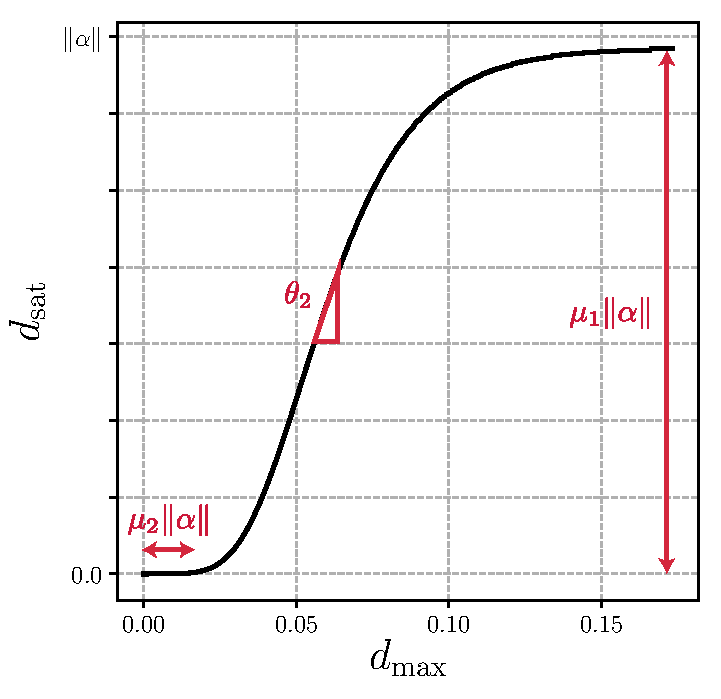
\includegraphics[width=.35\textwidth]{figures/dsat_edited}
	\vspace{-0.35cm}
	\caption{Pictorial description of the saturation function \eqref{eq:d_sat}. Note that when $d_{\rm max} = \|\alpha\|$ then $d_{\rm sat} = \mu_1\|\alpha\|$.}\label{fig:d_sat}%
\end{figure}

\begin{figure}[t]
\centering
	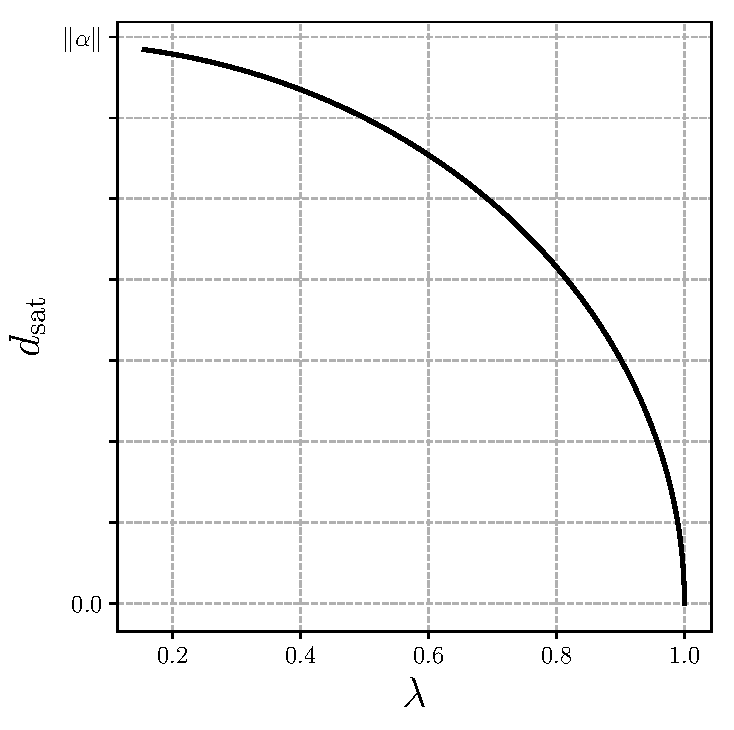
\includegraphics[width=.35\textwidth]{figures/decay_fcn}
	\vspace{-0.35cm}
	\caption{An illustration of the function defined in \eqref{eq:ph_index} showing a profile relatively quadratic for penalizing excursions inside $\mathcal{B}$.}\label{fig:ph_index}%
\end{figure}
%===============================================================================
\section{NUMERICAL RESULTS AND DISCUSSION}\label{sec:numerical_results}
This section is dedicated to describing the framework testbed and studies that demonstrate the effectiveness and efficiency of our control algorithm.
%===============================================================================
\subsection{Human-quadrotor benchmark}
%===============================================================================
\subsubsection{Robot}
Let us denote with $\{\mathcal{I}\}$ the inertial frame, and with $\{\mathcal{B}\}$ the body frame located at the center of mass (CoM) of the aerial vehicle. Consider a quadrotor with position $p = (x, y, z) \in \mathbb{R}^3$ expressed in $\{\mathcal{I}\}$, orientation $ \gamma = (\phi,\theta,\psi) \in \mathbb{R}^3$, linear velocity $v_b = (v_x, v_y, v_z) \in \mathbb{R}^3$ expressed in $\{\mathcal{B}\}$, angular rate $\omega = (\omega_x, \omega_y, \omega_z) \in \mathbb{R}^3$ expressed in $\{\mathcal{B}\}$ and rotational speed of the propellers $\Omega = (\Omega_1,\Omega_2,\Omega_3,\Omega_4) \in \mathbb{R}^4$, bounded by $\mathcal{X} = \{\Omega \in \mathbb{R}^4 \vcentcolon \ubar{\Omega} \leq \Omega \leq \Bar{\Omega}\}$. The system control inputs are the rotor torques, defined by $u \vcentcolon = (\tau_1,\tau_2,\tau_3,\tau_4) \in \mathbb{R}^4$ and constrained in magnitude $\mathcal{U} = \{u \in \mathbb{R}^4 \vcentcolon \ubar{u}\leq u \leq \Bar{u}\}$. Its nonlinear dynamics are then given by the first-order ordinary differential equations:
 \begin{equation}
 \dot{\xi} = f(\xi,u) = 
 \begin{pmatrix}
 	S^Tv_b \\
 	E \omega\\
	\frac{1}{m}F_b - R G - \omega\times v_b\\
	J^{-1}(M_b - \omega\times J\omega)\\
	\frac{1}{J_m}(u-C_D\Omega\odot\Omega-d\Omega)
\end{pmatrix}\label{eq:ode}%
 \end{equation}
 with state $\xi \vcentcolon = (p,\gamma,v_b,\omega,\Omega) \in \mathbb{R}^{16}$. The quadrotor's mass is denoted by $m$, $G =(0, 0, g) \in \mathbb{R}^3$ with $g$ being the gravitational acceleration, $d$ represents the drag coefficient of the rotor whose inertia is $J_m$. The element-wise product is denoted with $\odot$. The positive-definite matrix $J \in \mathbb{R}^{3 \times 3}$ denotes the vehicle inertia matrix. The rotation matrix from  $\{\mathcal{I}\}$ to $\{\mathcal{B}\}$ is represented by $S \in SO(3)$. Matrix $E \vcentcolon \mathbb{R}^3 \rightarrow \mathbb{R}^{3 \times 3}$ expresses the relation between the instantaneous rates of change of $\gamma$ and the instantaneous components of $\omega$. The total external forces and moments applied to the CoM of quadrotor and expressed in $\{\mathcal{B}\}$ are defined, respectively, as 
 \begin{equation}
 	\begin{aligned}
    F_b & \vcentcolon =  (0,0,F_z), \quad M_b \vcentcolon = (M_x, M_y, M_z)
	\end{aligned}
 \end{equation}
 with
 \begin{subequations}
 \begin{align}
 	F_z &= C_T(\Omega_{1}^{2}+\Omega_{2}^{2}+\Omega_{3}^{2}+\Omega_{4}^{2}),\label{eq:total_thrust}\\
 	M_x & = C_T\cdot l(\Omega_{2}^{2}-\Omega_{4}^{2}),\\
    M_y &= C_T\cdot l(\Omega_{3}^{2}-\Omega_{1}^{2}), \\
    M_z & = C_D(\Omega_{1}^{2}+\Omega_{3}^{2}-\Omega_{2}^{2}-\Omega_{4}^{2}),
 \end{align}
 \end{subequations}
where $C_T$ is the thrust coefficient, $C_D$ is the drag coefficient, and $l$ is the distance between the quadrotor's CoM and the rotor's center. As an example, we report  in Table \ref{tab:prm} the values of the  dynamic parameters appearing in \eqref{eq:ode} corresponding to the MikroKopter\footnote{\url{https://www.mikrokopter.de/en/home}} quadrotor platform.

\begin{table}[b]
\caption{MikroKopter physical parameters}
\centering
\begin{tabular}{lc}
\toprule
$m$ 	& $1.04$ kg \\
$l$ 	& $0.23$ m \\
$C_D$ 	& $10$ Nm/kHz$^2$ \\
$C_T$ 	& $595$ N/kHz$^2$ \\
$d$ 	& $0.5$ kN${\cdot}$m${\cdot}$s \\
$J_m$ 	& $0.08$ $\text{g}{\cdot}\text{m}^2$ \\
$J$ 	& $\text{diag}(0.01,0.01,0.07)$ $\text{kg}{\cdot}\text{m}^2$\\
\bottomrule
\end{tabular}\label{tab:prm}
\end{table}
%===============================================================================
\subsubsection{Reference trajectory}
The global planner provides a cartesian helical trajectory $\eta^r$ that avoids collisions with existing obstacles. This means that task variables are defined as $\eta \vcentcolon = p \in \mathbb{R}^3$. Note that the reference trajectory implicitly enforces safety.
 
%===============================================================================
\subsubsection{Pilot inputs}
Usually, pilots provide the quadrotor with the desired roll, pitch, $z$ angular rate, and total thrust, i.e., $g = (\phi_h,\theta_h,\omega_z, F_{z,h}) \in \mathbb{R}^4$. For simplicity, we assume that the desired $z$ angular rate is zero throughout the task, and the total thrust is mapped into the speed of the propellers, i.e., $\nu^r \vcentcolon g \mapsto \mathbb{R}^6$. To simulate the pilot inputs, we use a second NMPC controller that reads as follows:
\begin{equation}\label{eq:nlp}
{\!\!\!\!\!}{\!\!}\begin{aligned}
&\underset{\begin{subarray}{c}
\xi_0, \dots, \xi_N, \\
u_0, \dots, u_{N-1}
\end{subarray}}{\min} \frac{1}{2}\sum_{i=0}^{N-1} \Delta\eta_i^TQ_1\Delta\eta_i + \gamma_i^TQ_2\gamma_i + v_{b,i}^TQ_3v_{b,i} \\
&\,\,\,\,\,\,\,\,\,\,\,\,\,\,\,\,\,\,\,\,\, + \omega_i^TQ_4\omega_i + \Delta\Omega_i^TQ_5\Delta\Omega_i+u_i^TR_1u_i\\ 
& \,\,\,\,\,\,\,\,\,\,\,\,\,\,\,\,\,\,\,\, + \frac{1}{2}(\Delta\eta_N^TQ_{1N}\Delta\eta_N + \gamma_N^TQ_{2N}\gamma_N + v_{b,N}^TQ_{3N}v_{b,N} \\
&\,\,\,\,\,\,\,\,\,\,\,\,\,\,\,\,\,\,\,\,\, + \omega_N^TQ_{4N}\omega_N + \Delta\Omega_N^TQ_{5N}\Delta\Omega_N)\\
&\,\,\,\quad \text{s.t.} \,\,\,\,\,\,\,\,\, \eqref{eq:a}-\eqref{eq:d}.
\end{aligned}{\!\!\!}
\end{equation}
Here, $\Delta\Omega_i = (\Omega_i-\Omega_{\text{hovering}})$ for $i=0,\dots, N$ represents the propeller speed errors, where  $\Omega_{\text{hovering}} = \sqrt{(mg/4C_T)}$. The positive-definite weighting matrices are denoted by $Q_i, \,Q_{iN}$ for $i=1,\dots,5$ and $R_1$. In particular, constraint \eqref{eq:c} represents the control interface's real limitation. 

Once the solution of \eqref{eq:nlp} is computed, we can use the predicted state at stage $i=1$ as pilot inputs, namely
\begin{equation}
	\phi_h = \phi^\star, \quad \theta_h = \theta^\star, \quad \Omega_h = \Omega^\star,
\end{equation}
where the superscript $\star$ indicates the optimal solution.
\begin{remark} In practice, the total thrust coming from the joystick can be easily mapped into the propellers' desired speed and passed to the MI controller if one uses Eq. \eqref{eq:total_thrust} assuming hovering condition, i.e., $\Omega_{1} = \Omega_{2} = \Omega_{3} = \Omega_{4} = \Omega_{ss}$, which yields
\begin{equation*}
	\Omega_{ss} = \sqrt{\frac{F_{z,h}}{4C_T}}, \quad \Omega_h = \Omega_{ss}{\cdot}\mathbf{1_4}.
\end{equation*} 
\end{remark}
The distinction between pilots with a different skill level is made through the weighting matrices of the controller. Flying a quadrotor is less automated for novice pilots and for this reason requires more of their attention span than experienced ones. Due to their limited self-regulatory ability, their inputs tend to be oscillatory (lower values in the weighting matrices). In contrast, the inputs of experienced pilots tend to be more precise (higher values in the weighting matrices), presumably reflecting their ability to use perceptual cues to support their actions.

Moreover, as we need to predict human inputs to solve Problem \ref{problem:mi}, we adopt a zero-order hold (ZOH) method. This prediction method assumes that the future human inputs will all be the same as the current ones, an assumption that proved to be surprisingly effective in experimentation (see \cite{chipalkatty2013}).  
%===============================================================================
\subsubsection{Additional penalty terms}
As previously hypothesized, pilots would typically perform continuous maneuvers by changing their inputs all the time. To preserve smoothness in the generated trajectory, we consider additional penalty terms in the MI controller cost function. These terms rely on the following output functions:
\begin{equation}
	h(\xi_i) = h(\xi_N) = (\psi; v_b; \omega) \in \mathbb{R}^7
\end{equation}
and their corresponding references
\begin{equation}
	e_i = e_N = \mathbf{0_7}.
\end{equation}
The vector of zeros implies two underlying assumptions: first, we are not dealing with aggressive maneuvers; second, we assume it is an educated guess to initialize and, thereby, speed-up the subsequent optimization algorithm.
%===============================================================================
\subsubsection{NLPs parameterization}
Among several approaches available to discretize continuous-time OCPs, direct multiple shooting \cite{bock1984} will be used in this work due to its convergence and initialization properties. Additionally, we approximate the Hessian of the Lagrangian using the Generalized Gauss-Newton method so that structure-exploiting convex solvers can profit from the particular block-structure of the resulting quadratic program (QP).  

This endeavor's time horizon is $T$, which we divide into $N$ intervals so that we have the discrete-time step $\Delta t = T/N$. Assuming an equidistant grid and piecewise constant control parameterization, the following initial value problem defines the state trajectory $\xi(\pi)$ at each shooting interval:
\begin{equation}
	\dot{\xi}(\pi) = f(\pi,\xi(\pi),u_i), \quad \xi(t_i) = \xi_i, \quad \forall \pi \in [t_i, t_{i+1}].\label{eq:discrete_dyn}
\end{equation}
Function \eqref{eq:discrete_dyn} is evaluated numerically, $\xi(t_{i+1}) \approx F(\xi_i,u_i)$, using one step of explicit Runge Kutta 4th order per $\Delta t$.
%===============================================================================
%===============================================================================
\subsection{Implementation details}
\subsubsection{NMPC via real-time iteration scheme}
In real-time NMPC applications, (\textbf{NLP$_1$}) and (\textbf{NLP$_2$}) need to be solved at each sampling instant under the available computation time. To that end, we use a numerical strategy based on \emph{sequential quadratic programming} (SQP) that relies on the solution of a limited number of quadratic program (QP) subproblems, the so-called real-time iteration (RTI) scheme. More precisely, in this strategy only a single linearization and QP solve are carried out per sampling instant, leading to an approximate feedback control policy. An important ingredient in the RTI scheme is to keep the initial state as a constrained decision variable, which is often referred to as \emph{initial value embedding}. This allows one to divide computations into a preparation and a feedback phase, where the former is typically more expensive. In this work, we will be using the implementation of the RTI method by means of the high-performance software package \texttt{acados}.

The \emph{direct multiple shooting} approach is used in order to obtain (\textbf{NLP$_1$}) and (\textbf{NLP$_2$}). The state trajectories from stage 0 to $N$ are approximated using a numerical integration scheme, in this case an explicit Runge Kutta 4th order (ERK4), while the input trajectories are parametrized as piecewise constant. We make use of \texttt{acados} Python template-based interface to generate the libraries that implement (\textbf{NLP$_1$}) and (\textbf{NLP$_2$}), which are then wrapped by our mixed-initiative control algorithm, written in Python, which executes Algorithm 1. 

\IncMargin{1em}
\begin{algorithm}
\SetKwInOut{Input}{Input}\SetKwInOut{Output}{Output}
\Input{States $\Bar{\xi}_{0(k)},\Bar{\sigma}_{0(k)}$ and references $\Bar{\eta}_{(k)},\Tilde{\eta}_{(k)}$ at iteration $k$.}
\Output{Solution $(\sigma_i,u_i)_k$ for (\textbf{NLP$_2$}$)_k$ at iteration $k$.}
\KwData{maximum admissible error $a = (0.05,0.05,0.1)$ m, \textit{criterion}, simulation time $t_f$ = 6 s, sampling time $t_s = 0.015$ s.}
\BlankLine
\Begin{
	$k \longleftarrow 0$\;
	Calculate $\epsilon_a$ in \eqref{eq:aed}\;
	$\check{\epsilon} \longleftarrow 0$\;
	$\Hat{\epsilon} \longleftarrow \epsilon_a$\;
	\For{$k \longleftarrow 0$ \KwTo $t_f/t_s$}{
		Update $\Bar{\eta}_{(k)}$\;
		Solve (\textbf{NLP$_1$}$)_k$ for $\Bar{\xi}_{0(k)}$\;
		\For{$i \longleftarrow 0$ \KwTo $N$}{
			Calculate $\epsilon^\star_{i(k)}$ in \eqref{eq:ped}\;
		}
		\If{criterion = $(A_1)$}{
			\For{$i \longleftarrow N$ \KwTo $0$}{
				\If{$\epsilon^\star_{i(k)} < \Hat{\epsilon}$}{
      				$\Bar{N}_{i(k)} \longleftarrow \texttt{NaN}$\;
    			}
    			\Else{$\Bar{N}_{i(k)} \longleftarrow i$\;}{	
    			}
    		}
    		$\Bar{N}_{(k)} \longleftarrow$ last non-\texttt{NaN} element of $\Bar{N}_{i(k)}$\;
    		Evaluate zone-excursion function $\lambda_{A_1(k)}$ in \eqref{eq:lambda1}\;
    	}
    	\If{criterion = $(A_2)$}{
			\For{$i \longleftarrow N$ \KwTo $0$}{
				\If{$\epsilon^\star_{i(k)} > \Hat{\epsilon}$}{
      				$\epsilon^\star_{i(k)} \longleftarrow \Hat{\epsilon}$\;
    			}
    			$\epsilon^\star_{i,max(k)} \longleftarrow \epsilon^\star_{i(k)}$\;
    			
			}
			$\epsilon^\star_{max(k)} \longleftarrow \text{max}(\epsilon^\star_{i,max(k)})$\;
			Evaluate zone-excursion function $\lambda_{A_2(k)}$ in \eqref{eq:lambda2}\;
		}
		Build $W(\epsilon^\star_{i(k)})$ and ${W}_N(\epsilon^\star_{i(k)})$ in \eqref{eq:weight_matrices}\;
		Calculate $\mathcal{U}_{1(k)}$ and $\mathcal{U}_{2(k)}$ in \eqref{eq:control_law}\; 
		Simulate human commands based on $\mathbf{R}_{d(k)}$, $\mathcal{U}_{1(k)}$ and $\mathcal{U}_{2(k)}$\;
		Update $\Tilde{\eta}_{(k)}$\;
		Solve (\textbf{NLP$_2$}$)_k$ for $\Bar{\sigma}_{0(k)}$\;
		\Return $(\sigma_i, u_i)_k$
	}
}
\caption{zone NMPC for mixed-initiative control}\label{algo:zonenmpc}
\end{algorithm}\DecMargin{1em}
\subsubsection{Structure-exploiting QP solver and condensing approach}
The QP subproblems arising in the SQP algorithm in \texttt{acados} are addressed using the high-performance \texttt{HPIPM} \cite{frison2020} solver, which implements a primal-dual interior-point method. It is built on top of the linear algebra package \texttt{BLASFEO} \cite{frison2018}, finely tuned for multiple CPU architectures. This Riccati-based solver implements an efficient method for the solution of linear-quadratic (LQ) control problems, a special instance of equality constrained QP. Furthermore, \texttt{BLASFEO} is hardware-optimized for the moderately sized matrices present in our mixed-initiative NMPC. We use its \texttt{X64\_INTEL\_HASWELL} implementation, which exploits a set of vectorized instructions for the target CPU. Solution times are further reduced by reformulating the QPs resulting from our NMPC using the efficient partial condensing algorithm implemented in \texttt{HPIPM}. In particular, the algorithm finds the optimal level of sparsity for the solver, trading off horizon length for input vector size.
\subsection{Performance analysis}
%===============================================================================
\begin{figure}[h]
	\centering
	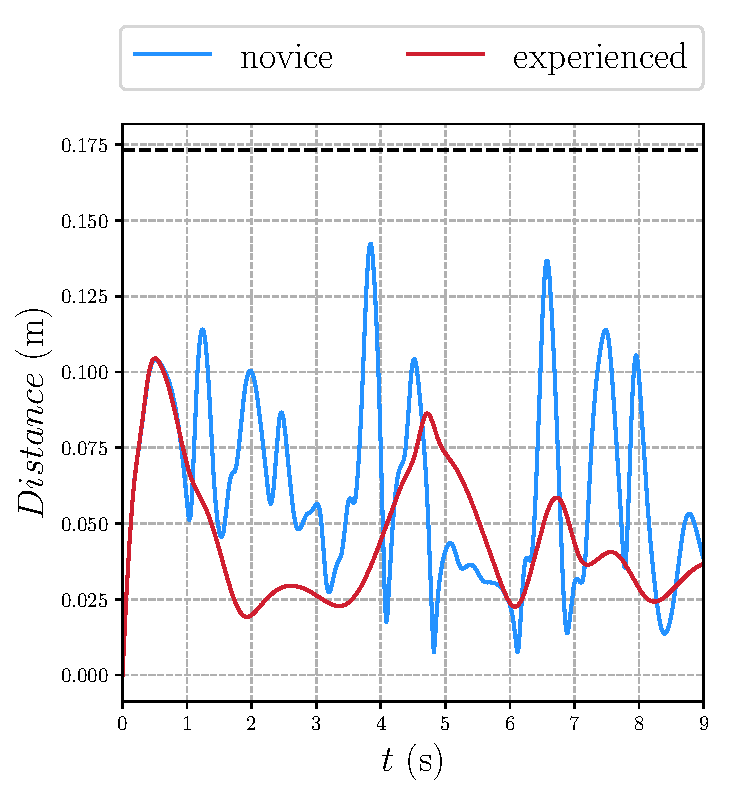
\includegraphics[width=0.4\textwidth]{figures/comparison}
	\vspace{-0.3cm}
	\caption{Distance between generated trajectories and reference; $\|\alpha\|$ is dashed.}\label{fig:boundary}%
\end{figure}
%===============================================================================
\begin{figure}[h]
	\centering
	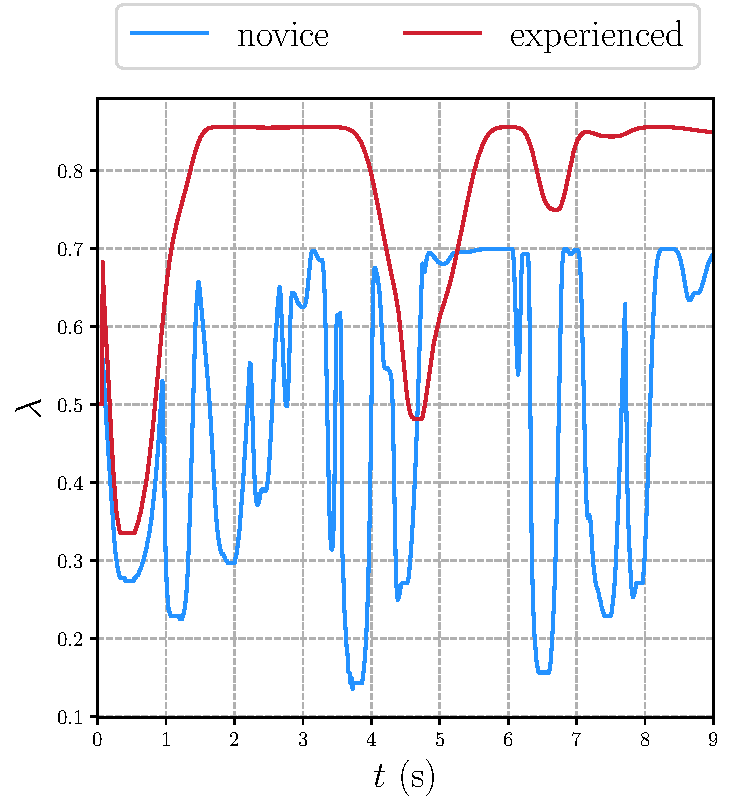
\includegraphics[width=0.38\textwidth]{figures/ph_index}
	\vspace{-0.3cm}
	\caption{Predicted healthiness index profiles indicating the level of human control authority.}\label{fig:ph_evo}%
\end{figure}
%===============================================================================
\begin{figure}[t]
	\centering
	\subfloat[Novice.]{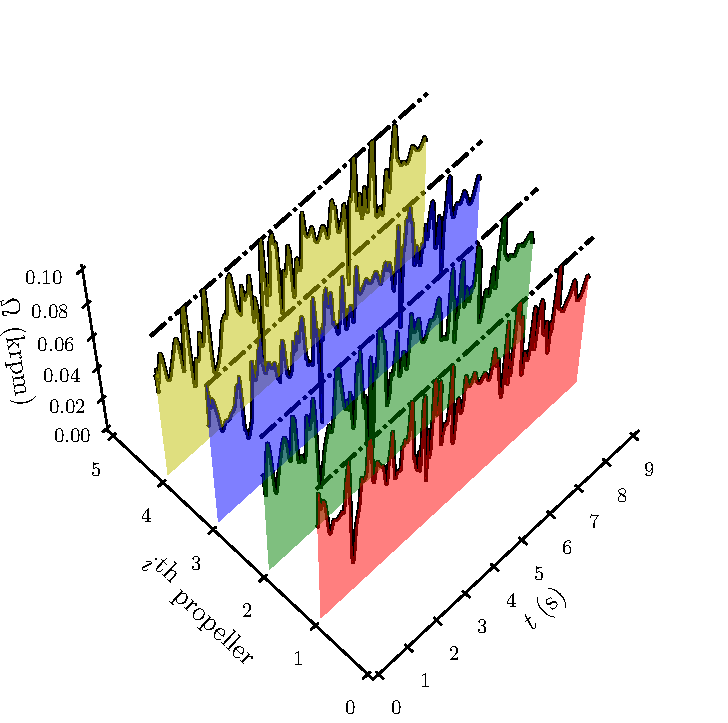
\includegraphics[width=0.4\textwidth]{figures/propeller_speed_novice}}\vspace{-0.39cm}
	\subfloat[Experienced.]{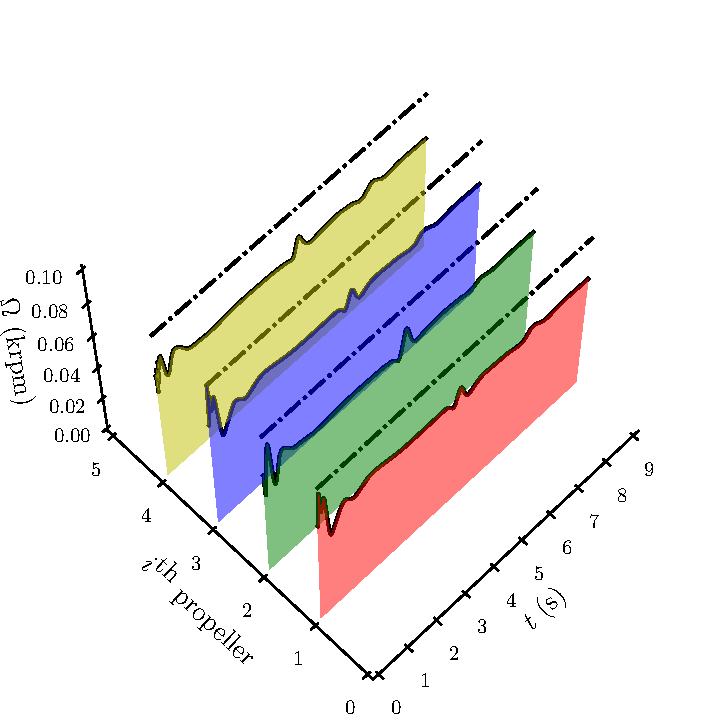
\includegraphics[width=0.4\textwidth]{figures/propeller_speed_experienced}}
	\caption{Generated propeller speeds; the upper bound $\bar{\Omega}$ is dashed.}\label{fig:prop_speed}%
\end{figure}
%===============================================================================
The proposed algorithm, that is, the blending mechanism and the mixed-initiative NMPC, use the parameters reported in Table \ref{tab:scenario1} in all test cases. In particular, we adopt a short virtual horizon $N_b$ to compensate for the fact that with a ZOH method, pilot inputs would have a natural tendency to violate the norm ball's boundary in the long run. The chosen value is a compromise between the base level of ``trust'' in the human inputs and the switching frequency of control authority. Another assumption made concerns the initialization of the blending mechanism. We assume that during the first iterations $\lambda = 0.5$, notably, none of the agents has control authority. Furthermore, the tests consider pilots with different competence levels. More specifically, the autonomous algorithm emulates a novice and an experienced pilot. This will enable a thorough follow-on comparative analysis of the control algorithm.    

Fig.~\ref{fig:output} displays the trajectories generated by our mixed-initiative NMPC for both pilots. The results show that our controller was able to maintain the quadrotor inside $\mathcal{B}$, successfully avoiding all obstacles in all cases (see Fig.~\ref{fig:boundary}). In Fig.~\ref{fig:human_inputs_s1}, we observe that the mixed-initiative NMPC commands closely follow the pilot inputs when the safety constraint is unlikely to be violated. This outcome is more evident for the experienced pilot, where the lines overlap almost completely, implying that the inputs issued kept the quadrotor closer to the reference trajectory. From Fig. \ref{fig:ph_evo}, it is obvious that the blending mechanism begins to drop off rapidly the level of control authority for the novice. At the same time, it maintains a relatively high level for the experienced pilot. Overall, note that the control algorithm assists the novice through what is often a very challenging part of their learning journey, the damping in pitching-rolling motions. The algorithm can keep up considerably with the signals' pattern (preserving the pilot's primary intentions), but attenuates their magnitude to cope with the safety constraint. Also, as the physical constraints herein regarded are linear, they can be enforced very efficiently by the optimization algorithm, as shown in Fig.~\ref{fig:prop_speed}.

Including maximum deviations provides versatility in the quadrotor motion generation. First, it gives a certain level of spatial freedom so that the quadrotor can leverage the motion by exploiting its dynamics. Second, it similarly adds new degrees of freedom to the controller. From a theoretic point of view, the control objective of the mixed-initiative NMPC can be seen as a target set (in the space of the task variables) instead of a target point, since inside $\mathcal{B}$ there are no preferences between one point and another \cite{camacho2010}.

The findings here indicate that our algorithm provides pilots with more control authority without sacrificing safety or even exceeding the robot's physical limits. Therefore, it has the potential to become a standard assistive scheme that can lead to a future improvement in pilot decision-making performance.

%===============================================================================
\begin{table}[h]
\caption{Parameters used by the blending mechanism and the mixed-initiative NMPC}
\centering
\begin{tabular}{cc|cc}
\toprule
$\ubar{\Omega}$ & $0$ & $\Bar{\Omega}$ & $0.09$ kHz \\
$\ubar{u}$ & $-0.1285$ Nm &  $\Bar{u}$ & $0.1285$ Nm \\
$T$ & $0.75$ s & $N$ & $50$ \\
$\alpha$ & $0.1{\cdot}\mathbf{1_3}$ m  & $N_b$ & $10$ \\
$\mu_1$ & 0.99 & $\mu_2$ & 0.3\\
$\theta_2$ & 50 & $\zeta$ & $1{\cdot}10^{-13}$\\
\midrule
\multicolumn{4}{c}{$Q_{\eta} = Q_{\eta_N} = \text{blkdiag}(250{\cdot}\mathbf{I_2}, 300)$, $Q_{\nu} = Q_{\nu_N} = 4{\cdot}10^3{\cdot}\mathbf{I_6}$,}\\
\multicolumn{4}{c}{$Q_{e} = Q_{e_N} = \text{blkdiag}(10, 3{\cdot}\mathbf{I_5}, 10)$, $R = 70{\cdot}\mathbf{I_4}$}\\
\bottomrule
\end{tabular}\label{tab:scenario1}
\end{table}
%===============================================================================

%\subsection{Performance analysis}
%In the simulations we assess the effectiveness of the mixed-initiative control algorithm in terms of whether or not human operators are afforded the freedom that is required to modify the reference tracked by the robot, regardless of the level of piloting skill. Additionally, we would like to measure the performance of the navigation task for the two adaptation criteria presented. Figure \ref{fig:l0_a1}--\ref{fig:l2_a2} show the results for six different simulations in which Algorithm 1 was used. Independently of the criterion used to compute $\lambda_{\bullet}$, the values $\lambda_{\bullet} = 0.0, \lambda_{\bullet} \in \mathbb{R} = (0.0,1.0), \lambda_{\bullet} = 1.0$ indicate \emph{fully automatic control}, \emph{shared control} and \emph{fully human control}, respectively.

The graphs depict the evolution of both zone-excursion functions $\lambda_{\bullet}$ for which the insets show the corresponding unfolding of either $\Bar{N}$ or $\epsilon^\star_{max}$. It is also shown the predicted Euclidean distances $\epsilon^\star_i$ analogous to the time interval of the inset. The light blue and pink colors in the graphs for criterion $(A_1)$ indicate the predicted Euclidian distances that are within and exceed the target zone, respectively, e.g. $\Bar{N} = 0$ and $\Bar{N} \in \mathbb{W} = [1,50]$. In contrast, for criterion $(A_2)$ pink corresponds to $\epsilon^\star_{max} \in \mathbb{R} = (0.0,1.0)$.

When $\Bar{N} \in \mathbb{W} = [1,50]$, i.e. PED exceeds the target zone, then $0 <\lambda_{A_1} \leq 1$, resulting in a reduction in the human control authority while $\lim_{\Bar{N}\to 50}\lambda_{A_1}(\Bar{N})$, according to \eqref{eq:weight_matrices}. In general, the insets of $\lambda_{A_1}$ show that, when active, the zone NMPC starts producing a precipitous fall in the human control authority. However, due to the high level of ``trust in the human" embedded in criterion $(A_1)$, this off-peak is short-lived. Because of the settling stage-weighting, the active shooting node is gradually decreased, with respect to previous NMPC solutions, right after the main $\lambda_{A_1}$ off-peak. This decrease corresponds to the transition from the shared control phase, in which $\epsilon^\star_i$ exceeds the target zone, to the phase fully controlled by the human, in which $\epsilon^\star_i$ undulates nonchalantly within $[\check{\epsilon},\Hat{\epsilon}]$, accruing no extra penalization, as $\Bar{N}$ remains equal to zero. 

On the other hand, when using criterion $(A_2)$, the zone NMPC persistently opts for stark shared control throughout the task. The aim of zone-excursion function $\lambda_{A_2}$ is to aggressively reduce human control authority only an increasing in the error margin arises, indicating that this is a criterion with a low level of ``trust in the human". Maximum PED-weighting constantly attenuates human control authority compared with using the fixed nominal weights and, for this reason, is inherently safer as it is ``active" at each prediction step.

The simulation results have shown that the proposed mixed-initiative control algorithm is able to provide to the human operator the freedom to modify the reference tracked by the robot, no matter the level of piloting skill. Proposed zone NMPC with criterion $(A_1)$ yields an oscillatory, albeit slightly more sluggish, return to the target zone. Instead, proposed zone NMPC with criterion $(A_2)$ does not exceed the target zone whatsoever. As maximum PED-weighting ends up being continuously ``active", it is advantageous for more challenging situations, for instance, with an inexperienced pilot, capable of reducing the human workload and also providing higher performance benefits.

%%%%%%%%%%%%%%%%%%%%%%%%%%%%%%%%%%%%%%%%%%%%%%%%%%%%%%%%%%%%%%%%%%%%%%%%%%%%%%%%%%%%%%
%%%%%%%%%%%%%%%%%%%%%%%%%%%%%%%%%%%%%%%%%%%%%%%%%%%%%%%%%%%%%%%%%%%%%%%%%%%%%%%%%%%%%%
\newpage
\paragraph{Inexperienced $(\mathbf{L0})$:} Closed-loop results for mixed-initiative control algorithm.
\begin{figure*}[h]\centering
	\includegraphics[width=1.0\textwidth]{../../Software/plots/case0/noob/position}
	\caption{Using adaptation criterion ($A_1$).}\label{fig:l0_a1}%
	\vspace{0.5cm}
	\includegraphics[width=1.0\textwidth]{../../Software/plots/case1/noob/position}
	\caption{Using adaptation criterion ($A_2$).}\label{fig:l0_a2}%
\end{figure*}
%%%%%%%%%%%%%%%%%%%%%%%%%%%%%%%%%%%%%%%%%%%%%%%%%%%%%%%%%%%%%%%%%%%%%%%%%%%%%%%%%%%%%%
\newpage
\paragraph{Intermediate $(\mathbf{L1})$:} Closed-loop results for mixed-initiative control algorithm.
\begin{figure*}[h]\centering
	\includegraphics[width=1.0\textwidth]{../../Software/plots/case0/inter/position}
	\caption{Using adaptation criterion ($A_1$).}\label{fig:l1_a1}%
	\vspace{0.5cm}
	\includegraphics[width=1.0\textwidth]{../../Software/plots/case1/inter/position}
	\caption{Using adaptation criterion ($A_2$).}\label{fig:l1_a2}%
\end{figure*}
%%%%%%%%%%%%%%%%%%%%%%%%%%%%%%%%%%%%%%%%%%%%%%%%%%%%%%%%%%%%%%%%%%%%%%%%%%%%%%%%%%%%%%
\newpage
\paragraph{Experienced $(\mathbf{L2})$:} Closed-loop results for mixed-initiative control algorithm.
\begin{figure*}[h]\centering
	\includegraphics[width=1.0\textwidth]{../../Software/plots/case0/pro/position}
	\caption{Using adaptation criterion ($A_1$).}\label{fig:l2_a1}%
	\vspace{0.5cm}
	\includegraphics[width=1.0\textwidth]{../../Software/plots/case1/pro/position}
	\caption{Using adaptation criterion ($A_2$).}\label{fig:l2_a2}%
\end{figure*}
%%%%%%%%%%%%%%%%%%%%%%%%%%%%%%%%%%%%%%%%%%%%%%%%%%%%%%%%%%%%%%%%%%%%%%%%%%%%%%%%%%%%%%
%%%%%%%%%%%%%%%%%%%%%%%%%%%%%%%%%%%%%%%%%%%%%%%%%%%%%%%%%%%%%%%%%%%%%%%%%%%%%%%%%%%%%%
%\subsection{Stability}
%\input{content/stability}
\subsection{Computational burden}
Solution times reported are from an Intel Core i5-4288U @ 2.6 GHz running macOS Catalina. Simulations showed that \texttt{HPIPM} is significantly faster in solving the partially condensed QP arising in the NMPC formulation than the corresponding dense QP. The average times per SQP-iteration in \texttt{acados} were $4.27$ ms for the novice and $3.87$ ms for the experienced pilot. It is interesting to note that one can modify $N_b$ and potentially improve the blending mechanism performance without affecting solution times significantly. Fig.~\ref{fig:violin} shows that all quantities appear to be related to $N$ rather than $N_b$.

As previously mentioned, partial condensing is an approach in-between the sparse and the condensed one. Here, in particular, the horizon length can be reduced at the expense of a larger input vector. This degree of freedom is used to find the best subproblem size for \texttt{HPIPM}. Thus, given the dimensions of the resulting QP subproblems in our controller, computational efficiency is granted through partial condensing as it allows us to exploit hardware throughput better.

\begin{figure}[t]
	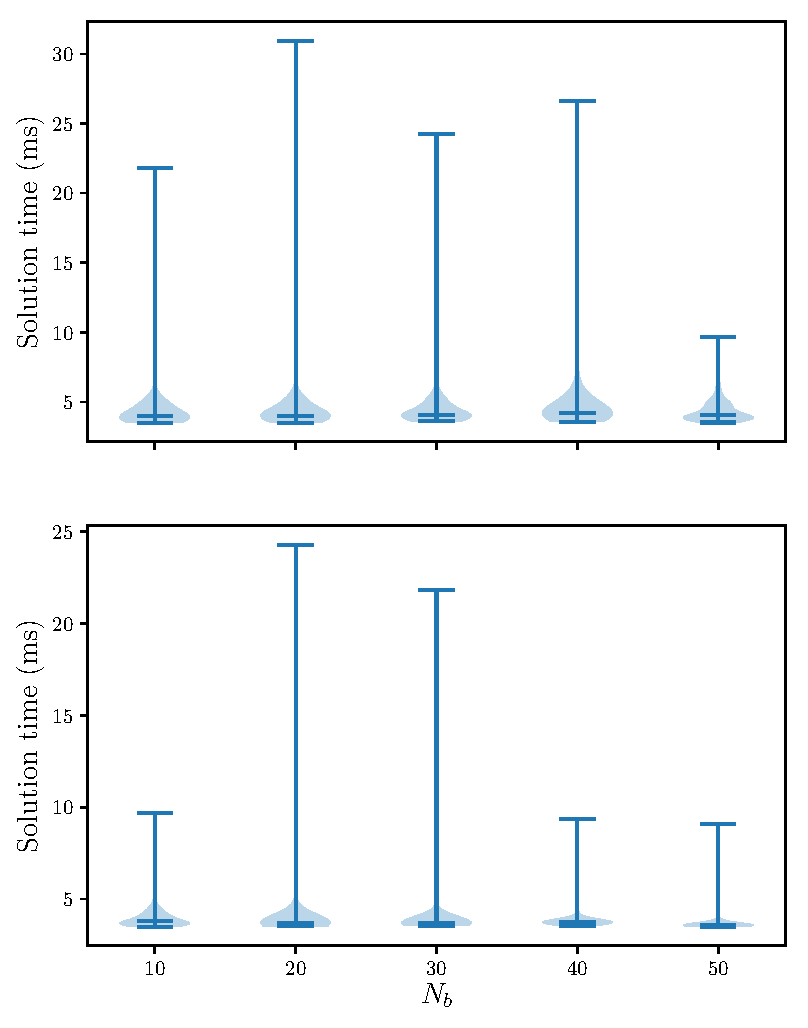
\includegraphics[width=0.5\textwidth]{figures/violin}
	\vspace{-0.8cm}
	\caption{Violin plot representations of the solution times associated with the mixed-initiative controller in simulations with a novice (top) and an experienced pilot (bottom). Central bars represent the median values for each virtual horizon $N_b$.}\label{fig:violin}
\end{figure}
%===============================================================================
\section{CONCLUSIONS}\label{sec:conclusion}
In this paper, we have presented a new mixed-initiative NMPC controller for enforcing safety in human-quadrotor interactions. We adopt a predict-then-blend framework to mix human inputs and motion generator commands during operation. Through the quadrotor's predicted positions, we assess whether safety rules are met to perform then the blending, a mechanism designed to continuously measure the violation of the rules. The presented controller uses an efficient RTI-based scheme that iteratively refines the combined commands to fulfill all intrinsic constraints within the available computation time. In simulation, we evaluate our controller's performance against an autonomous algorithm that emulates the behavior of pilots with different competence levels. The results show that the control scheme allows safety enforcement with specific benefits for useful assistance to pilots, especially novices, and low computational effort. Thanks to high-performance software implementations, we can speed-up our controller's solution times, demonstrating efficient computational performance. Future work will focus on evaluating the pilot's cognitive load through real-world experiments.
%\addtolength{\textheight}{-12cm}  
%===============================================================================
\bibliographystyle{IEEEtran}
\bibliography{biblio}
%===============================================================================
\end{document}
